\documentclass{report}

\usepackage[T2A]{fontenc}
\usepackage[utf8]{luainputenc}
\usepackage[english, russian]{babel}
\usepackage[pdftex]{hyperref}
\usepackage[14pt]{extsizes}
\usepackage{listings}
\usepackage{color}
\usepackage{geometry}
\usepackage{enumitem}
\usepackage{multirow}
\usepackage{graphicx}
\usepackage{indentfirst}
\usepackage{hyperref}
\graphicspath{ {../../modules/task_1/Abuyassen_A_CSR/images/} }
\geometry{a4paper,top=2cm,bottom=3cm,left=2cm,right=1.5cm}
\setlength{\parskip}{0.5cm}
\setlist{nolistsep, itemsep=0.3cm,parsep=0pt}

\lstset{language=C++,
basicstyle=\footnotesize,
keywordstyle=\color{blue}\ttfamily,
stringstyle=\color{red}\ttfamily,
commentstyle=\color{green}\ttfamily,
morecomment=[l][\color{magenta}]{\#},
tabsize=4,
breaklines=true,
breakatwhitespace=true,
title=\lstname,
}

\makeatletter
\renewcommand\@biblabel[1]{#1.\hfil}
\makeatother

\begin{document}

\begin{titlepage}

\begin{center}
Министерство науки и высшего образования Российской Федерации
\end{center}

\begin{center}
Федеральное государственное автономное образовательное учреждение высшего образования \\
Национальный исследовательский Нижегородский государственный университет им. Н.И. Лобачевского
\end{center}

\begin{center}
Институт информационных технологий, математики и механики
\end{center}

\vspace{4em}

\begin{center}
\textbf{\LargeОтчет по лабораторной работе} \\
\end{center}
\begin{center}
\textbf{\Large«Умножение разреженных матриц. Элементы комплексного типа. Формат хранения матрицы – строковый (CRS)»} \\
\end{center}

\vspace{4em}

\newbox{\lbox}
\savebox{\lbox}{\hbox{text}}
\newlength{\maxl}
\setlength{\maxl}{\wd\lbox}
\hfill\parbox{7cm}{
\hspace*{5cm}\hspace*{-5cm}\textbf{Выполнил:} \\ студент группы 381908-4 \\ Абуяссен Албара\\
\\
\hspace*{5cm}\hspace*{-5cm}\textbf{Проверил:}\\ доцент кафедры МОСТ, \\ кандидат технических наук \\ Сысоев А.В.\\
}
\vspace{\fill}

\begin{center} Нижний Новгород \\ 2022 \end{center}

\end{titlepage}

\setcounter{page}{2}

% Содержание
\tableofcontents
\newpage

% Введение
\section*{Введение}
Разреженная матрица или разреженный массив — это матрица, в которой большинство элементов равны нулю. Концепция разреженности полезна в комбинаторике и прикладных областях, таких как теория сетей и численный анализ, которые обычно имеют низкую плотность значимых данных или связей. Большие разреженные матрицы часто появляются в научных или инженерных приложениях при решении дифференциальных уравнений в частных производных. При хранении и манипулировании разреженными матрицами на компьютере полезно и часто необходимо использовать специализированные алгоритмы и структуры данных, которые используют преимущества разреженной структуры матрицы. этот отчет содержит решение для эффективного хранения разреженных матриц с использованием типа хранения разреженных матриц-строковой вместе с умножением матриц с использованием технологий параллельного программирования TBB (Threading Building Blocks) и Openmp.
\addcontentsline{toc}{section}{Введение}

% Постановка задачи
\section*{Постановка задачи}
\addcontentsline{toc}{section}{Постановка задачи}
для реализации задачи необходимо:
\begin{enumerate}
\item Понимание структуры данных CSR и необходимости ее использования.
\item Изучение способов реализации CSR.
\item Понимание того, как реализовать транспонирование CSR.
\item Понимание реализации последовательного умножения CSR.
\item Изучение технологий параллельного программирования TBB и Openmp.
\item Изменение алгоритма умножения для поддержки параллельной реализации с меньшей синхронизацией, насколько это возможно.
\end{enumerate}

\newpage

% Описание алгоритмов
\section*{Описание алгоритмов}
\addcontentsline{toc}{section}{Описание алгоритмов}
\begin{enumerate}
\item Алгоритм преобразования разреженной матрицы в формат CSR: 
\newline пусть A будет разреженной матрицей размера M * N, чтобы преобразовать ее в формат CSR, нам нужно перебрать все элементы, сначала перебрав все строки A от 0 до M-1, и внутри этого цикла нам нужно перебрать все элементы i-й строки от 0 до N-1. Всякий раз, когда мы находим ненулевой элемент, мы добавляем его в вектор <Values>, который сохраняет все ненулевые элементы матрицы A, и добавляем номер j-го столбца в вектор <cols\textunderscore index>, который сохраняет номера столбцов всех ненулевых элементов. и после каждого цикла j мы добавляем накопленную сумму ненулевых элементов, которые мы нашли до сих пор, к вектору <row\textunderscore ptr>.
\item Алгоритм транспонирования матрицы формата CSR:
Пусть A будет разреженной матрицей, преобразованной в формат CSR. чтобы найти транспонирование $A^{T}$, мы должны:
\begin{enumerate}
\item Создать пустую структуру CSR для получения результата операции транспонирования с заменой значений количества строк и столбцов и инициализировать вектор <rowнакопленную сумму ненулевых элементов, которые мы нашли до сих пор, к вектору <row\textunderscore ptr> для получения одного дополнительного элемента.
\item Цикл от 0 до числа ненулевых элементов-1 и счетчик внутри вектора <row\textunderscore ptr> будет столбцом.
\item Цикл от 2 до размера вектора <row\textunderscore ptr> и создание нового сдвинутого вектора <row\textunderscore ptr> путем создания добавочной суммы.
\item зациклить каждую строку матрицы и вычислить новый индекс каждого элемента в конечной структуре операции, а затем сохранить лемму и ее номер столбца в окончательной структуре.
\end{enumerate}
\item Алгоритм реализации умножения формата CSR:
\newline пусть A и B — матрицы размерностей M*N и T*Z соответственно, отформатированные в CSR. для реализации умножения A*B мы должны:
\begin{enumerate}
\item Проверить правильность размеров обеих матриц (N==T).
\item Найти $B^{T}$ транспонирование матрицы B.
\item Цикл по всем строкам матрицы A. и внутри этого цикла мы создаем еще один цикл для перебора всех ненулевых элементов i-й строки.
\item Если в i-й строке существуют ненулевые элементы, то на итерации мы возьмем элемент, и номер его столбца мы переберем все строки $B^{T}$, и каждую итерацию мы переберем все ненулевые элементы j-й строки $B^{T}$.
\item Если номер столбца элемента i-й строки A равен номеру столбца элемента j-й строки $B^{T}$, то мы вычисляем умножение этих элементов и сохраняем конечный продукт в i-й строке j-й столбец итоговой матрицы.
\end{enumerate}
\end{enumerate}

% Схема распараллеливания
\section*{Схема распараллеливания}
\addcontentsline{toc}{section}{Схема распараллеливания}
\par для реализации параллельного программирования в операции умножения мы делим номер внешнего цикла между потоками. К счастью, TBB и Openmp позаботятся об этой задаче, единственное, что нам осталось сделать, это гарантировать лучшую производительность, гарантируя, что все потоки будут выполнять почти одинаковый объем работы, потому что не всегда стандартный способ планирования задачи дает ожидаемую производительность.
\newpage

% Описание программной реализации
\section*{Описание программной реализации}
\addcontentsline{toc}{section}{Описание программной реализации}
\par Оператор умножения структуры CSR реализует последовательную операцию, сначала перебирая все строки первой матрицы, и каждая i-я итерация выбирает все ненулевые элементы i-й строки A и вычисляет скалярное произведение каждой строки Матрица $B^{T}$, а затем сохранить результат в i-й строке j-й столбец итоговой матрицы.
\begin{lstlisting}
const std::vector < std::complex < int >> operator * (const CSR & A, const CSR & B)
\end{lstlisting}
\subsection*{OpenMP}
\addcontentsline{toc}{subsection}{OpenMP}
\par Используя \verb|#pragma omp parallel for|, мы можем разделить итерации внешнего цикла (количество строк A) между потоками, и здесь мы можем захотеть изменить тип планирования (по умолчанию статический) на динамический, потому что в некоторых случаях статическое планирование помещает некоторые потоки. на большее количество работы, чем другие, что приводит к снижению производительности в результате
\begin{lstlisting}
#pragma omp parallel
  {
    if (dynamic) {
      omp_set_schedule(omp_sched_dynamic, 1);
    } else {
      int chunk_size = A.rows / omp_get_num_threads();
      omp_set_schedule(omp_sched_static, chunk_size);
    }
    #pragma omp for schedule(runtime)
      for (int i = 0; i < A.rows; i++) {
\end{lstlisting}
примечание: функция \verb|omp_set_schedule| не поддерживается в Visual Studio
\newpage

\subsection*{TBB}
\addcontentsline{toc}{subsection}{TBB}
\par Для TBB используется \verb|tbb::parallel_for|, который просматривает общий диапазон итераций для выполнения, предоставленный объектом \newline \verb|tbb::blocked_range<int>|. Он разбивает эту сумму на ряд поддиапазонов, которые распределяются как задачи для выполнения рабочими потоками.
\begin{lstlisting}
  tbb::parallel_for(tbb::blocked_range < int > (0, A.rows),
    [ & ](tbb::blocked_range < int > r) {
      for (int i = r.begin(); i < r.end(); i++)
\end{lstlisting}

\newpage

% Подтверждение корректности
\section*{Подтверждение корректности}
\addcontentsline{toc}{section}{Подтверждение корректности}
Для проверки правильности реализации были написаны гугл-тесты, которые генерируют случайные разреженные матрицы разного размера и запускают как последовательную, так и параллельную реализацию и подсчитывают время работы каждой из них. в результате, если окончательные матрицы параллельной и последовательной реализаций равны, тесты будут пройдены.
\newpage

% Результаты экспериментов
\section*{Результаты экспериментов}
\addcontentsline{toc}{section}{Результаты экспериментов}
\par Эксперименты для оценки эффективности проводились на ноутбук со следующими характеристиками:

\begin{itemize}
\item Процессор: Intel® Core™ i5-8250U Processor
\item Оперативная память: 20 ГБ;
\item ОС: Ubuntu 20.04 LTS
\end{itemize}
\par Замеры параллельных версий производились на 8 потоках.

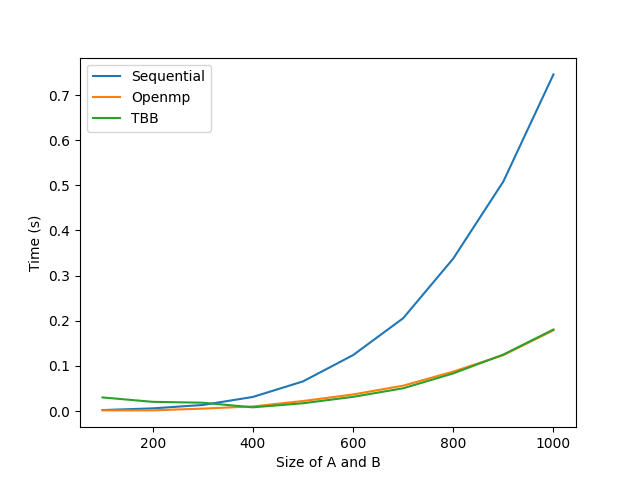
\includegraphics{result}

\par Время работы TBB и openmp было почти равным. но ясно, что параллельная реализация была действительно эффективной

\newpage

% Заключение
\section*{Заключение}
\addcontentsline{toc}{section}{Заключение}
в этом отчете мы увидели, как сохранить разреженную матрицу в формате CSR и реализовать операцию умножения. Мы также увидели, как использовать технологии параллельного программирования TBB и Openmp и их огромное влияние на скорость работы.

\newpage

% Список литературы
\begin{thebibliography}{1}
\addcontentsline{toc}{section}{Список литературы}
\bibitem Sparse Matrix and its representations | Set 1 (Using Arrays and Linked Lists).
\url{https://www.geeksforgeeks.org/sparse-matrix-representation/}
\bibitem Introduction to OpenMP - Tim Mattson (Intel).
\newline \url{https://www.youtube.com/playlist?list=PLLX-Q6B8xqZ8n8bwjGdzBJ25X2utwnoEG}
\end{thebibliography}
\newpage

% Приложение
\section*{Приложение}
\addcontentsline{toc}{section}{Приложение}
\par Последовательная версия
\par \verb|1.CSR.h|
\begin{lstlisting}

#include <vector>
#include <complex>

struct CSR {
  std::vector<std::complex<int>> values;
  std::vector < int > row_ptr;
  std::vector < int > cols_index;
  int rows;
  int cols;
  int NNZ;

    friend const std::vector < std::complex < int >>
    operator*(const CSR &A, const CSR &B);
    friend const bool operator==(const CSR &A, const CSR &B);
};

CSR sparesify(const std::vector < std::complex < int >>  &M,
 int height, int width);
CSR sparse_transpose(const CSR &input);
std::vector < std::complex < int >> tbb_multiply(const CSR & A,
  const CSR & B);
std::vector < std::complex < int >>  randomSparseMatrix(int N, int M);

\end{lstlisting}
\par \verb|2.CSR.cpp|
\begin{lstlisting}
#include "CSR.h"
#include <vector>
#include <random>
#include <complex>

CSR sparesify(const std::vector < std::complex < int >> & M,
  int height, int width) {
  CSR new_csr;
  new_csr.rows = height;
  new_csr.cols = width;
  new_csr.row_ptr.push_back(0);
  new_csr.NNZ = 0;
  for (int i = 0; i < new_csr.rows; i++) {
    for (int j = 0; j < new_csr.cols; j++) {
      if (M[i * width + j] != 0) {
        new_csr.values.push_back(M[i * width + j]);
        new_csr.cols_index.push_back(j);
        new_csr.NNZ++;
      }
    }
    new_csr.row_ptr.push_back(new_csr.NNZ);
  }

  return new_csr;
}

CSR sparse_transpose(const CSR & input) {
  CSR res {
      std::vector < std::complex < int >> (input.NNZ, 0),
      std::vector < int > (input.cols + 2, 0),  // one extra
      std::vector < int > (input.NNZ, 0),
      input.cols,
      input.rows,
      input.NNZ
  };

  // count per column
  for (int i = 0; i < input.NNZ; ++i) {
    ++res.row_ptr[input.cols_index[i] + 2];
  }

  // from count per column generate new rowPtr (but shifted)
  for (size_t i = 2; i < res.row_ptr.size(); ++i) {
    // create incremental sum
    res.row_ptr[i] += res.row_ptr[i - 1];
  }

  // perform the main part
  for (int i = 0; i < input.rows; ++i) {
    for (int j = input.row_ptr[i]; j < input.row_ptr[i + 1]; ++j) {
      // calculate index to transposed matrix
      // at which we should place current element,
      // and at the same time build final rowPtr
      const int new_index = res.row_ptr[input.cols_index[j] + 1]++;
      res.values[new_index] = input.values[j];
      res.cols_index[new_index] = i;
    }
  }
  res.row_ptr.pop_back();  // pop that one extra

  return res;
}

const std::vector < std::complex < int >> operator * (const CSR & A,
  const CSR & B) {
  if (A.cols != B.rows)
    throw "Size Error";
  CSR B_t = sparse_transpose(B);
  std::vector < std::complex < int >> result(A.rows * B.cols, 0);
  for (int i = 0; i < A.rows; i++)
    for (int j = A.row_ptr[i]; j < A.row_ptr[i + 1]; j++) {
      int Ai = A.cols_index[j];
      std::complex < int > Avalue = A.values[j];
      for (int k = 0; k < B_t.rows; k++) {
        std::complex < int > sum(0, 0);
        for (int l = B_t.row_ptr[k]; l < B_t.row_ptr[k + 1]; l++)
          if (Ai == B_t.cols_index[l]) {
            sum += Avalue * B_t.values[l];
            break;
          }
        if (sum != std::complex < int > (0, 0)) {
          result[i * B_t.rows + k] += sum;
        }
      }
    }
  return result;
}

const bool operator == (const CSR & A,
  const CSR & B) {
  return A.values == B.values && A.cols_index == B.cols_index &&
  A.row_ptr == B.row_ptr && A.rows == B.rows
  && A.cols == B.cols && A.NNZ == B.NNZ;
}

std::vector < std::complex < int >> randomSparseMatrix(int N, int M) {
  std::random_device dev;
  std::mt19937 gen(dev());
  std::vector < std::complex < int >> result(N * M, 0);
  for (int i = 0; i < N; i++) {
    for (int j = 0; j < M; j++) {
      if (gen() % 100 == 0) {
        result[i * M + j] += std::complex < int > (gen() % 10, gen() % 10);
      }
    }
  }

  return result;
}
\end{lstlisting}
\par \verb|3.main.cpp|
\begin{lstlisting}
#include <gtest/gtest.h>
#include <vector>
#include <complex>
#include "./CSR.h"

typedef std::vector<std::vector<std::complex<int>>> matrix;
typedef std::complex<int> element;

TEST(CSR_seq, can_create_a_matrix_and_sparesify_it) {
    matrix A = {
        {0, element(1, 3)},
        {0, 0},
        {element(5, 5), 0},
    };
    CSR A_ = sparesify(A);
    std::vector<std::complex<int>> check = {element(1, 3), element(5, 5)};
    ASSERT_TRUE(A_.values == check);
}

TEST(CSR_seq, can_get_transpose) {
    matrix A = {
        {0, element(1, 3)},
        {0, 0},
        {element(5, 5), 0},
    };

    CSR A_ = sparesify(A);
    CSR A_t = sparse_transpose(A_);

    CSR check {
        {element(5, 5), element(1, 3)},
        {0, 1, 2},
        {2, 0},
        2,
        3,
        2
    };

    ASSERT_TRUE(A_t == check);
}

TEST(CSR_seq, can_multiply) {
    matrix A = {
        {0, element(1, 3)},
        {0, 0},
        {element(5, 5), 0},
    };
    CSR A_ = sparesify(A);

    matrix B = {
        {0, element(2, 4)},
        {element(1, 3), 0},
    };
    CSR B_ = sparesify(B);

    matrix result = A_ * B_;

    matrix check = {
        {element(-8, 6), 0},
        {0, 0},
        {0, element(-10, 30)},
    };
    ASSERT_TRUE(result == check);
}

TEST(CSR_seq, multiplication_throws_exception) {
    matrix A = {
        {0, element(1, 3)},
        {0, 0},
        {element(5, 5), 0},
    };
    CSR A_ = sparesify(A);

    matrix B = {
        {0, element(2, 4)},
        {element(1, 3), 0},
        {0, 0},
    };
    CSR B_ = sparesify(B);
    EXPECT_ANY_THROW(A_ * B_);
}

TEST(CSR_seq, can_multiply_random_matrix) {
    matrix A = randomSparseMatrix(4, 3);
    CSR A_ = sparesify(A);

    matrix B = randomSparseMatrix(3, 4);
    CSR B_ = sparesify(B);
    EXPECT_NO_THROW(A_ * B_);
}

int main(int argc, char **argv) {
    ::testing::InitGoogleTest(&argc, argv);
    return RUN_ALL_TESTS();
}
\end{lstlisting}

\par OpenMP Версия
\par \verb|1.CSR_omp.h|
\begin{lstlisting}
#include <vector>
#include <complex>

struct CSR {
  std::vector<std::complex<int>> values;
  std::vector < int > row_ptr;
  std::vector < int > cols_index;
  int rows;
  int cols;
  int NNZ;

    friend const std::vector < std::complex < int >>
    operator*(const CSR &A, const CSR &B);
    friend const bool operator==(const CSR &A, const CSR &B);
};

CSR sparesify(const std::vector < std::complex < int >>  &M,
 int height, int width);
CSR sparse_transpose(const CSR &input);
std::vector < std::complex < int >> omp_multiply(const CSR & A,
  const CSR & B, bool dynamic = false);
std::vector < std::complex < int >>  randomSparseMatrix(int N, int M);
\end{lstlisting}
\par \verb|2.CSR_omp.cpp|
\begin{lstlisting}
#include "CSR_omp.h"
#include <omp.h>
#include <vector>
#include <random>
#include <complex>

CSR sparesify(const std::vector < std::complex < int >> & M,
  int height, int width) {
  CSR new_csr;
  new_csr.rows = height;
  new_csr.cols = width;
  new_csr.row_ptr.push_back(0);
  new_csr.NNZ = 0;
  for (int i = 0; i < new_csr.rows; i++) {
    for (int j = 0; j < new_csr.cols; j++) {
      if (M[i * width + j] != 0) {
        new_csr.values.push_back(M[i * width + j]);
        new_csr.cols_index.push_back(j);
        new_csr.NNZ++;
      }
    }
    new_csr.row_ptr.push_back(new_csr.NNZ);
  }

  return new_csr;
}

CSR sparse_transpose(const CSR & input) {
  CSR res {
      std::vector < std::complex < int >> (input.NNZ, 0),
      std::vector < int > (input.cols + 2, 0),  // one extra
      std::vector < int > (input.NNZ, 0),
      input.cols,
      input.rows,
      input.NNZ
  };

  // count per column
  for (int i = 0; i < input.NNZ; ++i) {
    ++res.row_ptr[input.cols_index[i] + 2];
  }

  // from count per column generate new rowPtr (but shifted)
  for (size_t i = 2; i < res.row_ptr.size(); ++i) {
    // create incremental sum
    res.row_ptr[i] += res.row_ptr[i - 1];
  }

  // perform the main part
  for (int i = 0; i < input.rows; ++i) {
    for (int j = input.row_ptr[i]; j < input.row_ptr[i + 1]; ++j) {
      // calculate index to transposed matrix
      // at which we should place current element,
      // and at the same time build final rowPtr
      const int new_index = res.row_ptr[input.cols_index[j] + 1]++;
      res.values[new_index] = input.values[j];
      res.cols_index[new_index] = i;
    }
  }
  res.row_ptr.pop_back();  // pop that one extra

  return res;
}

const std::vector < std::complex < int >> operator * (const CSR & A,
  const CSR & B) {
  if (A.cols != B.rows)
    throw "Size Error";
  CSR B_t = sparse_transpose(B);
  std::vector < std::complex < int >> result(A.rows * B.cols, 0);
  for (int i = 0; i < A.rows; i++)
    for (int j = A.row_ptr[i]; j < A.row_ptr[i + 1]; j++) {
      int Ai = A.cols_index[j];
      std::complex < int > Avalue = A.values[j];
      for (int k = 0; k < B_t.rows; k++) {
        std::complex < int > sum(0, 0);
        for (int l = B_t.row_ptr[k]; l < B_t.row_ptr[k + 1]; l++)
          if (Ai == B_t.cols_index[l]) {
            sum += Avalue * B_t.values[l];
            break;
          }
        if (sum != std::complex < int > (0, 0)) {
          result[i * B_t.rows + k] += sum;
        }
      }
    }
  return result;
}

const bool operator == (const CSR & A,
  const CSR & B) {
  return A.values == B.values && A.cols_index == B.cols_index &&
  A.row_ptr == B.row_ptr && A.rows == B.rows
  && A.cols == B.cols && A.NNZ == B.NNZ;
}

std::vector < std::complex < int >> randomSparseMatrix(int N, int M) {
  std::random_device dev;
  std::mt19937 gen(dev());
  std::vector < std::complex < int >> result(N * M, 0);
  for (int i = 0; i < N; i++) {
    for (int j = 0; j < M; j++) {
      if (gen() % 100 == 0) {
        result[i * M + j] += std::complex < int > (gen() % 10, gen() % 10);
      }
    }
  }

  return result;
}

std::vector < std::complex < int >> omp_multiply(const CSR & A,
  const CSR & B, const bool dynamic) {
  if (A.cols != B.rows)
    throw "Size error";
  CSR B_t = sparse_transpose(B);
  std::vector < std::complex < int >> result(A.rows * B.cols, 0);
  #pragma omp parallel
  {
    if (dynamic) {
      omp_set_schedule(omp_sched_dynamic, 1);
    } else {
      int chunk_size = A.rows / omp_get_num_threads();
      omp_set_schedule(omp_sched_static, chunk_size);
    }
    #pragma omp for schedule(runtime)
    for (int i = 0; i < A.rows; i++) {
      for (int j = A.row_ptr[i]; j < A.row_ptr[i + 1]; j++) {
        int Ai = A.cols_index[j];
        std::complex < int > Avalue = A.values[j];
        for (int k = 0; k < B_t.rows; k++) {
          std::complex < int > sum(0, 0);
          for (int l = B_t.row_ptr[k]; l < B_t.row_ptr[k + 1]; l++)
            if (Ai == B_t.cols_index[l]) {
              sum += Avalue * B_t.values[l];
              break;
            }
          if (sum != std::complex < int > (0, 0)) {
            result[i * B_t.rows + k] += sum;
          }
        }
      }
    }
  }
  return result;
}
\end{lstlisting}
\par \verb|3.main.cpp|
\begin{lstlisting}
#include <gtest/gtest.h>
#include <omp.h>
#include <vector>
#include <complex>
#include "./CSR_omp.h"

TEST(CSR_seq, multiplication_100_100) {
    int width = 100, height = 100;
    std::vector<std::complex<int>> A = randomSparseMatrix(height, width);
    std::vector<std::complex<int>> B = randomSparseMatrix(height, width);
    CSR A_ = sparesify(A, height, width);
    CSR B_ = sparesify(B, height, width);
    double dtime;
    dtime = omp_get_wtime();
    std::vector<std::complex<int>> SEQ = A_ * B_;
    dtime = omp_get_wtime() - dtime;
    printf("Sequential time : %f s\n", dtime);
    dtime = omp_get_wtime();
    std::vector<std::complex<int>> PAR = omp_multiply(A_, B_, false);
    dtime = omp_get_wtime() - dtime;
    printf("Parallel time : %f s\n", dtime);
    dtime = omp_get_wtime();
    ASSERT_TRUE(SEQ == PAR);
}

TEST(CSR_seq, multiplication_250_300) {
    int width = 300, height = 250;
    std::vector<std::complex<int>> A = randomSparseMatrix(height, width);
    std::vector<std::complex<int>> B = randomSparseMatrix(width, height);
    CSR A_ = sparesify(A, height, width);
    CSR B_ = sparesify(B, width, height);
    double dtime;
    dtime = omp_get_wtime();
    std::vector<std::complex<int>> SEQ = A_ * B_;
    dtime = omp_get_wtime() - dtime;
    printf("Sequential time : %f s\n", dtime);
    dtime = omp_get_wtime();
    std::vector<std::complex<int>> PAR = omp_multiply(A_, B_, false);
    dtime = omp_get_wtime() - dtime;
    printf("Parallel time : %f s\n", dtime);
    dtime = omp_get_wtime();
    ASSERT_TRUE(SEQ == PAR);
}

TEST(CSR_seq, multiplication_1000_1000) {
    int width = 1000, height = 1000;
    std::vector<std::complex<int>> A = randomSparseMatrix(height, width);
    std::vector<std::complex<int>> B = randomSparseMatrix(width, height);
    CSR A_ = sparesify(A, height, width);
    CSR B_ = sparesify(B, width, height);
    double dtime;
    dtime = omp_get_wtime();
    std::vector<std::complex<int>> SEQ = A_ * B_;
    dtime = omp_get_wtime() - dtime;
    printf("Sequential time : %f s\n", dtime);
    dtime = omp_get_wtime();
    std::vector<std::complex<int>> PAR = omp_multiply(A_, B_, false);
    dtime = omp_get_wtime() - dtime;
    printf("Parallel time : %f s\n", dtime);
    dtime = omp_get_wtime();
    ASSERT_TRUE(SEQ == PAR);
}

TEST(CSR_seq, multiplication_250_160) {
    int width = 160, height = 250;
    std::vector<std::complex<int>> A = randomSparseMatrix(height, width);
    std::vector<std::complex<int>> B = randomSparseMatrix(width, height);
    CSR A_ = sparesify(A, height, width);
    CSR B_ = sparesify(B, width, height);
    double dtime;
    dtime = omp_get_wtime();
    std::vector<std::complex<int>> SEQ = A_ * B_;
    dtime = omp_get_wtime() - dtime;
    printf("Sequential time : %f s\n", dtime);
    dtime = omp_get_wtime();
    std::vector<std::complex<int>> PAR = omp_multiply(A_, B_, false);
    dtime = omp_get_wtime() - dtime;
    printf("Parallel time : %f s\n", dtime);
    dtime = omp_get_wtime();
    ASSERT_TRUE(SEQ == PAR);
}

TEST(CSR_seq, multiplication_20_10) {
    int width = 20, height = 10;
    std::vector<std::complex<int>> A = randomSparseMatrix(height, width);
    std::vector<std::complex<int>> B = randomSparseMatrix(width, height);
    CSR A_ = sparesify(A, height, width);
    CSR B_ = sparesify(B, width, height);
    double dtime;
    dtime = omp_get_wtime();
    std::vector<std::complex<int>> SEQ = A_ * B_;
    dtime = omp_get_wtime() - dtime;
    printf("Sequential time : %f s\n", dtime);
    dtime = omp_get_wtime();
    std::vector<std::complex<int>> PAR = omp_multiply(A_, B_, false);
    dtime = omp_get_wtime() - dtime;
    printf("Parallel time : %f s\n", dtime);
    dtime = omp_get_wtime();
    ASSERT_TRUE(SEQ == PAR);
}

int main(int argc, char **argv) {
    ::testing::InitGoogleTest(&argc, argv);
    return RUN_ALL_TESTS();
}
\end{lstlisting}

\par TBB версия
\par \verb|1.CSR_tbb.h|
\begin{lstlisting}
#include <vector>
#include <complex>

struct CSR {
  std::vector<std::complex<int>> values;
  std::vector < int > row_ptr;
  std::vector < int > cols_index;
  int rows;
  int cols;
  int NNZ;

    friend const std::vector < std::complex < int >>
    operator*(const CSR &A, const CSR &B);
    friend const bool operator==(const CSR &A, const CSR &B);
};

CSR sparesify(const std::vector < std::complex < int >>  &M,
 int height, int width);
CSR sparse_transpose(const CSR &input);
std::vector < std::complex < int >> tbb_multiply(const CSR & A,
  const CSR & B);
std::vector < std::complex < int >>  randomSparseMatrix(int N, int M);
\end{lstlisting}
\par \verb|2.CSR_tbb.cpp|
\begin{lstlisting}
#include "CSR_tbb.h"
#include <tbb/tbb.h>
#include <vector>
#include <random>
#include <complex>

CSR sparesify(const std::vector < std::complex < int >> & M,
  int height, int width) {
  CSR new_csr;
  new_csr.rows = height;
  new_csr.cols = width;
  new_csr.row_ptr.push_back(0);
  new_csr.NNZ = 0;
  for (int i = 0; i < new_csr.rows; i++) {
    for (int j = 0; j < new_csr.cols; j++) {
      if (M[i * width + j] != 0) {
        new_csr.values.push_back(M[i * width + j]);
        new_csr.cols_index.push_back(j);
        new_csr.NNZ++;
      }
    }
    new_csr.row_ptr.push_back(new_csr.NNZ);
  }

  return new_csr;
}

CSR sparse_transpose(const CSR & input) {
  CSR res {
      std::vector < std::complex < int >> (input.NNZ, 0),
      std::vector < int > (input.cols + 2, 0),  // one extra
      std::vector < int > (input.NNZ, 0),
      input.cols,
      input.rows,
      input.NNZ
  };

  // count per column
  for (int i = 0; i < input.NNZ; ++i) {
    ++res.row_ptr[input.cols_index[i] + 2];
  }

  // from count per column generate new rowPtr (but shifted)
  for (size_t i = 2; i < res.row_ptr.size(); ++i) {
    // create incremental sum
    res.row_ptr[i] += res.row_ptr[i - 1];
  }

  // perform the main part
  for (int i = 0; i < input.rows; ++i) {
    for (int j = input.row_ptr[i]; j < input.row_ptr[i + 1]; ++j) {
      // calculate index to transposed matrix
      // at which we should place current element,
      // and at the same time build final rowPtr
      const int new_index = res.row_ptr[input.cols_index[j] + 1]++;
      res.values[new_index] = input.values[j];
      res.cols_index[new_index] = i;
    }
  }
  res.row_ptr.pop_back();  // pop that one extra

  return res;
}

const std::vector < std::complex < int >> operator * (const CSR & A,
  const CSR & B) {
  if (A.cols != B.rows)
    throw "Size Error";
  CSR B_t = sparse_transpose(B);
  std::vector < std::complex < int >> result(A.rows * B.cols, 0);
  for (int i = 0; i < A.rows; i++)
    for (int j = A.row_ptr[i]; j < A.row_ptr[i + 1]; j++) {
      int Ai = A.cols_index[j];
      std::complex < int > Avalue = A.values[j];
      for (int k = 0; k < B_t.rows; k++) {
        std::complex < int > sum(0, 0);
        for (int l = B_t.row_ptr[k]; l < B_t.row_ptr[k + 1]; l++)
          if (Ai == B_t.cols_index[l]) {
            sum += Avalue * B_t.values[l];
            break;
          }
        if (sum != std::complex < int > (0, 0)) {
          result[i * B_t.rows + k] += sum;
        }
      }
    }
  return result;
}

const bool operator == (const CSR & A,
  const CSR & B) {
  return A.values == B.values && A.cols_index == B.cols_index &&
  A.row_ptr == B.row_ptr && A.rows == B.rows
  && A.cols == B.cols && A.NNZ == B.NNZ;
}

std::vector < std::complex < int >> randomSparseMatrix(int N, int M) {
  std::random_device dev;
  std::mt19937 gen(dev());
  std::vector < std::complex < int >> result(N * M, 0);
  for (int i = 0; i < N; i++) {
    for (int j = 0; j < M; j++) {
      if (gen() % 100 == 0) {
        result[i * M + j] += std::complex < int > (gen() % 10, gen() % 10);
      }
    }
  }

  return result;
}

std::vector < std::complex < int >> tbb_multiply(const CSR & A,
  const CSR & B) {
  if (A.cols != B.rows)
    throw "Size error";
  CSR B_t = sparse_transpose(B);
  std::vector < std::complex < int >> result(A.rows * B.cols, 0);
  tbb::parallel_for(tbb::blocked_range < int > (0, A.rows),
    [ & ](tbb::blocked_range < int > r) {
      for (int i = r.begin(); i < r.end(); i++)
        for (int j = A.row_ptr[i]; j < A.row_ptr[i + 1]; j++) {
          int Ai = A.cols_index[j];
          std::complex < int > Avalue = A.values[j];
          for (int k = 0; k < B_t.rows; k++) {
            std::complex < int > sum(0, 0);
            for (int l = B_t.row_ptr[k]; l < B_t.row_ptr[k + 1]; l++)
              if (Ai == B_t.cols_index[l]) {
                sum += Avalue * B_t.values[l];
                break;
              }
            if (sum != std::complex < int > (0, 0)) {
              result[i * B_t.rows + k] += sum;
            }
          }
        }
    });
  return result;
}
\end{lstlisting}
\par \verb|3.main.cpp|
\begin{lstlisting}
#include <gtest/gtest.h>
#include <tbb/tick_count.h>
#include <vector>
#include <complex>
#include "./CSR_tbb.h"

TEST(CSR_tbb, multiplication_100_100) {
    int width = 100, height = 100;
    std::vector<std::complex<int>> A = randomSparseMatrix(height, width);
    std::vector<std::complex<int>> B = randomSparseMatrix(height, width);
    CSR A_ = sparesify(A, height, width);
    CSR B_ = sparesify(B, height, width);
    tbb::tick_count t0, t1;
    t0 = tbb::tick_count::now();
    std::vector<std::complex<int>> SEQ = A_ * B_;
    t1 = tbb::tick_count::now();
    printf("Sequential time : %g s\n", (t1-t0).seconds());
    t0 = tbb::tick_count::now();
    std::vector<std::complex<int>> PAR = tbb_multiply(A_, B_);
    t1 = tbb::tick_count::now();
    printf("Parallel time : %g s\n", (t1-t0).seconds());
    ASSERT_TRUE(SEQ == PAR);
}

TEST(CSR_tbb, multiplication_250_300) {
    int width = 300, height = 250;
    std::vector<std::complex<int>> A = randomSparseMatrix(height, width);
    std::vector<std::complex<int>> B = randomSparseMatrix(width, height);
    CSR A_ = sparesify(A, height, width);
    CSR B_ = sparesify(B, width, height);
    tbb::tick_count t0, t1;
    t0 = tbb::tick_count::now();
    std::vector<std::complex<int>> SEQ = A_ * B_;
    t1 = tbb::tick_count::now();
    printf("Sequential time : %g s\n", (t1-t0).seconds());
    t0 = tbb::tick_count::now();
    std::vector<std::complex<int>> PAR = tbb_multiply(A_, B_);
    t1 = tbb::tick_count::now();
    printf("Parallel time : %g s\n", (t1-t0).seconds());
    ASSERT_TRUE(SEQ == PAR);
}

TEST(CSR_tbb, multiplication_1000_1000) {
    int width = 1000, height = 1000;
    std::vector<std::complex<int>> A = randomSparseMatrix(height, width);
    std::vector<std::complex<int>> B = randomSparseMatrix(width, height);
    CSR A_ = sparesify(A, height, width);
    CSR B_ = sparesify(B, width, height);
    tbb::tick_count t0, t1;
    t0 = tbb::tick_count::now();
    std::vector<std::complex<int>> SEQ = A_ * B_;
    t1 = tbb::tick_count::now();
    printf("Sequential time : %g s\n", (t1-t0).seconds());
    t0 = tbb::tick_count::now();
    std::vector<std::complex<int>> PAR = tbb_multiply(A_, B_);
    t1 = tbb::tick_count::now();
    printf("Parallel time : %g s\n", (t1-t0).seconds());
    ASSERT_TRUE(SEQ == PAR);
}

TEST(CSR_tbb, multiplication_250_160) {
    int width = 160, height = 250;
    std::vector<std::complex<int>> A = randomSparseMatrix(height, width);
    std::vector<std::complex<int>> B = randomSparseMatrix(width, height);
    CSR A_ = sparesify(A, height, width);
    CSR B_ = sparesify(B, width, height);
    tbb::tick_count t0, t1;
    t0 = tbb::tick_count::now();
    std::vector<std::complex<int>> SEQ = A_ * B_;
    t1 = tbb::tick_count::now();
    printf("Sequential time : %g s\n", (t1-t0).seconds());
    t0 = tbb::tick_count::now();
    std::vector<std::complex<int>> PAR = tbb_multiply(A_, B_);
    t1 = tbb::tick_count::now();
    printf("Parallel time : %g s\n", (t1-t0).seconds());
    ASSERT_TRUE(SEQ == PAR);
}

TEST(CSR_tbb, multiplication_20_10) {
    int width = 20, height = 10;
    std::vector<std::complex<int>> A = randomSparseMatrix(height, width);
    std::vector<std::complex<int>> B = randomSparseMatrix(width, height);
    CSR A_ = sparesify(A, height, width);
    CSR B_ = sparesify(B, width, height);
    tbb::tick_count t0, t1;
    t0 = tbb::tick_count::now();
    std::vector<std::complex<int>> SEQ = A_ * B_;
    t1 = tbb::tick_count::now();
    printf("Sequential time : %g s\n", (t1-t0).seconds());
    t0 = tbb::tick_count::now();
    std::vector<std::complex<int>> PAR = tbb_multiply(A_, B_);
    t1 = tbb::tick_count::now();
    printf("Parallel time : %g s\n", (t1-t0).seconds());
    ASSERT_TRUE(SEQ == PAR);
}

int main(int argc, char **argv) {
    ::testing::InitGoogleTest(&argc, argv);
    return RUN_ALL_TESTS();
}
\end{lstlisting}
\end{document}
